%!TEX root = ../hr-paper.tex
\section{Method} % (fold)
\label{sec:method}

This section will show what methods where used to segment the dataset. It will do so in a chronological order based on the example image shown in section \ref{sec:dataset} in figure \ref{fig:dataset:chinese:example}.

\subsection{Segmentation}

\subsubsection{Rotation and binarization}


As discussed in the introduction (\ref{sec:introduction}) the Chinese characters were supplied in greyscale strokes of characters in the western orientation (from left to right).

In order to segment the characters from an image a combination of methods were used. First the image is binarized. Binarization is done by applying a Gaussian filter on the image to remove some of the pixel noise. Then Otsu's \cite{otsu}  method of finding a threshold is used. The image is then binarized using this threshold.

After binarization the image is rotated. This is done because most images in the dataset are titled slightly. As discussed in the dataset section (\ref{sec:dataset}) This is probably due to some variations in the orientation of the paper during the scanning process. Rotation is done by resizing the image in the vertical direction to half its size. The idea behind this is that the characters will be squeezed together and form a horizontal line, this line can then be used to find the optimal rotation. This is done by taking the horizontal densities. The maximum densities are saved for the different rotations (between $+1\degree$ and $-1\degree$). The rotation with the largest maximum density is where the line is likely to be the most horizontal. This is taken as the optimal rotation. The image is rotated with this optimal angle.

\subsubsection{Vertical location}

\begin{figure}[ht]
  \centering
  \begin{subfigure}{0.49\textwidth}
    \centering
    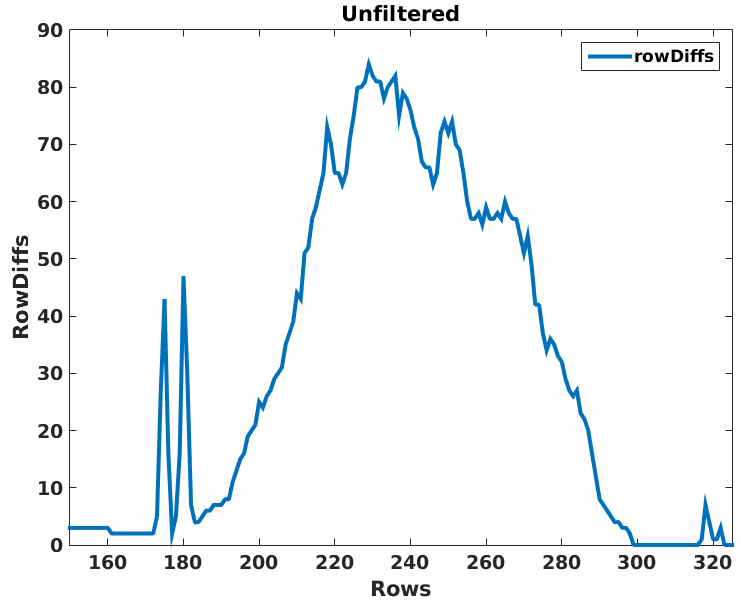
\includegraphics[width=\textwidth]{./images/method/unfiltered.png}
    \caption{Unfiltered density changes}
    \label{fig:method:unfiltered}
  \end{subfigure}
  \begin{subfigure}{0.49\textwidth}
    \centering
    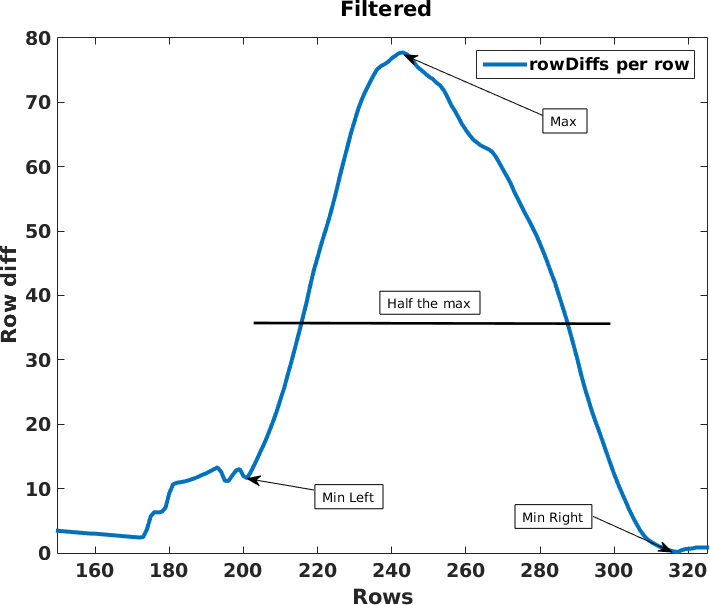
\includegraphics[width=\textwidth]{./images/method/filtered.png}
    \caption{Filtered density changes}
    \label{fig:method:filtered}
  \end{subfigure}
  \caption{Method of finding the vertical location of the characters}
  \label{fig:method:vertical:location}
\end{figure}

After the characters are rotated the location of the characters is determined on the vertical axes. The used method to determine this location is horizontal projection on the changes in pixels from black to white. On the densities an averaging filter is first applied. Each row is averaged with ten of its neighbor rows. To illustrate this the changes in densities were taken on the example image shown in the dataset section (\ref{fig:dataset:chinese:example}). The effect of the averaging is clearly visible in figure \ref{fig:method:vertical:location}. In figure \ref{fig:method:unfiltered} the unfiltered image is show. The plot has many peaks and also the top black line is clearly visible in the densities on the left side of the image. In figure \ref{fig:method:filtered} the filtered image is shown. Only the global peaks stay and the noise peak from the black line has almost disappeared.


\begin{figure}[ht]
  \begin{minipage}{\linewidth}
    \centering
    \[S=\left[\begin{array}{ccc}
		-1 & 0 & 1
    \end{array}\right]\]
  \end{minipage}%
  \caption{Sobel opperator}
  \label{mat:method:sobel}
\end{figure}

In order to find the location of the characters, the global maximum of changes in densities is taken. This is always the top of the highest peak of the characters. To find the bases on both sides of the peak a Sobel operator is used (shown in figure \ref{mat:method:sobel}). Sobel's operators can be used to find the gradient in a signal, demonstrated in a paper by Richard O. Duda and Peter E. Hart (\cite{Duda}) and later by Sobel self (\cite{Sobel}). To find these minima The half of the max is taken and from this half the first occurrence where the gradient crosses zero in the left and right direction is taken as a base of the mountain. The half of the max is used because on the top of the plot sometimes goes up and down even with the average filtering. The half max makes sure the whole height of the characters is taken. After determining the vertical location of the characters the image is cropped accordingly. Whitespace on the left and right side of the image is also removed.

\begin{figure}[ht]
  \centering
  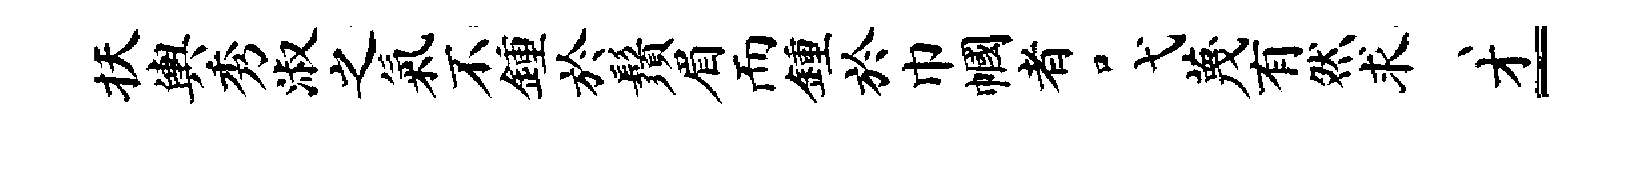
\includegraphics[width=\textwidth]{./images/method/trimmed.png}
  \caption{Rotated and cropped image}
  \label{fig:method:vertical:cropped}
\end{figure}

\subsubsection{Connected components}

We are left with the row of characters. An example is shown in figure \ref{fig:method:vertical:cropped}. This image is rotated and cropped from figure \ref{fig:dataset:chinese:example}. In order to find the characters in this row the connected components are taken. These are taken with the method described by Sedgewick (\cite{Sedgewick}). Sedgewick's method will give us a list of all the connected components in the image. If multiple components are above each other we assume that these components are part of the same character. These components are merged. Some components are not directly on top of each-other. It is determent how much the components overlap vertically. If the overlapping width is larger or the same as $0.4$ times the width of the smaller of the two components, they are merged. This is done to make sure the components are on top of each other and not some small part of one component is on top of an other component.

After merging vertically we are left with a list of components that might be outliers in terms of width in comparison with the mean width of the characters in the supplied labeled dataset. In order to recognize outliers the mean and standard deviation was calculated from the characters in the labeled dataset, also shown in section \ref{sec:dataset} and table \ref{tab:dataset:metrics}. A component is deemed a small out-lier if:

\begin{equation}
C_w < \mu_{lw} + 2 \sigma_{lw} 
\end{equation}

\noindent and a big out-lier if:

\begin{equation}
C_w > \mu_{lw} + 2 \sigma_{lw} 
\end{equation}

Here $C_w$ is the component's width, $\mu_{lw}$ is the mean width ,and $\sigma_{lw}$ is the standard deviation in width. Both were taken from the labels of the dataset

Small component can be noise or a character. A small component is more likely to be a character if it has an big amount of whitespace left and right from it. Except when it is the first or the last component in the list. To check for this the amount of whitespace on both sides of the small component is measured and added to the with of that component. If the component is the first or the last component in the list the white space is only measured on one side and is added twice to the width. With the added with the component reevaluated for being an out-lier.

The list with components still holds noise components. There are different types of noise present in the images. This algorithm tries to find unwanted `blobs' and too small components. The unwanted `blobs' are detected by taking the square of the component and filling it with white pixels. The component itself is then printed on this square in black pixels. The component in determined to be noise if the rectangle consists of more than 40 percent black pixels. This number is based on the labels of the dataset where the amount of black pixels in the rectangle was always lower than 40 percent of the pixels. This method removes components like the black bar shown in figure \ref{fig:method:vertical:cropped} on the outer right side of the image. An image is deemed noise if the width of the character is smaller than 15 pixels. 

The small components that are left in the list are now merged with the smallest of its two neighbor components. If a neighboring component is deemed big a small component will not be merged with it. If a component has a big neighbor to the left and a big neighbor to the right, This small component will not be merged. After each merger the components widths will be evaluated. If two merged components are still small, the algorithm will try to merge them again with one of the (new) smallest neighbors.

After merging all small components are dealt with. The component list still contains big out-liers. Some might even been created during merging. These components are spitted by projecting the variations in white pixels to black pixels (or the amount of fluctuations in white pixels). Where there are less variations there is more white space. The characters are split on where the fluctuations of the whitespace is minimal. After splitting the components are reevaluated on width. If a component is determined big it is split again. This is done until the component is not big anymore.


\subsubsection{Finding the character box}

With the split big components the segmentation part is completed. In order to validate the segmented images the location of the characters need to be determined in the original image. Because the image is rotated before segmentation the locations of the segmented images need to be rotated to point to the correct location in the original image. The location of the segmented characters is given by taking the $x$,$y$,$width$ and $height$ variables. This creates a rectangle on the original image where a character is determined to be. But because the characters outputted by the segmentation system are (merged) connected components there might be parts of other characters present in the rectangle that are not present in the character outputted by the segmentation system.

The approximation of the rectangle is made by calculating  all corner coordinates of the rectangle by taking the max and min row and column of the characters in the rotated image. Then these coordinates are rotated with the following formulas:

\begin{equation}
    x' = y \times sin(\alpha) + x \times cos(\alpha)
\end{equation}

\begin{equation}
    y' = y \times cos(\alpha) - x \times sin(\alpha)
\end{equation}

After rotating the minimum value for $x'$ and $y'$ is taken to determine the upper left corner of the rectangle. Then the width is determined by:

\begin{equation}
    width = abs(min(x_1,x_2,x_3,x_4) - max(x_1,x_2,x_3,x_4))
\end{equation}

The height is calculated in a similar fashion:

\begin{equation}
    height = abs(min(y_1,y_2,y_3,y_4) - max(y_1,y_2,y_3,y_4))
\end{equation}

These equations give the $x$,$y$,$width$ and $height$ variables needed to reconstruct the rectangle. After approximating the rectangle the characters are saved for use in the feature extractor and later the classifier of the character segmentation system.

\subsection{Feature Extraction}

%simple feature extraction

Because the focus of this system lies on the segmentation and the classification a simple feature extractor was designed. The feature extractor uses boxing and edge detection to construct 22 features.

Each character image is divided into four boxes. (inspired by ... paper) Per box the edges in four directions are calculated with a Sobel or a Prewit filter.

\begin{figure}[ht]
  \begin{minipage}{0.24\linewidth}
    \centering
    \[\left[\begin{array}{ccc}
    -1 & 0 & 1\\
    -1 & 0 & 1\\
    -1 & 0 & 1\\
    \end{array}\right]\]
    \subcaption{$S_{Vertical}$}
  \end{minipage}%
    \begin{minipage}{0.24\linewidth}
    \centering
    \[\left[\begin{array}{ccc}
    -1 & -1 & -1\\
    0 & 0 & 0\\
    1 & 1 & 1\\
    \end{array}\right]\]
    \subcaption{$S_{Horizontal}$}
  \end{minipage}%
    \begin{minipage}{0.24\linewidth}
    \centering
    \[\left[\begin{array}{ccc}
    -1 & -1 & 0\\
    -1 & 0 & 1\\
    0 & 1 & 1\\
    \end{array}\right]\]
    \subcaption{$S_{diagonal-left}$}
  \end{minipage}%
    \begin{minipage}{0.24\linewidth}
    \centering
    \[\left[\begin{array}{ccc}
    0 & -1 & -1\\
    1 & 0 & -1\\
    1 & 1 & 0\\
    \end{array}\right]\]
    \subcaption{$S_{diagonal-right}$}
  \end{minipage}%
  \caption{Sobel opperator in four directions.}
  \label{mat:method:sobel:2d}
\end{figure}

\begin{figure}[ht]
  \begin{minipage}{0.24\linewidth}
    \centering
    \[\left[\begin{array}{ccc}
    -1 & 0 & 1\\
    -2 & 0 & 2\\
    -1 & 0 & 1\\
    \end{array}\right]\]
    \subcaption{$P_{Vertical}$}
  \end{minipage}%
    \begin{minipage}{0.24\linewidth}
    \centering
    \[\left[\begin{array}{ccc}
    -1 & -2 & -1\\
    0 & 0 & 0\\
    1 & 2 & 1\\
    \end{array}\right]\]
    \subcaption{$P_{Horizontal}$}
  \end{minipage}%
    \begin{minipage}{0.24\linewidth}
    \centering
    \[\left[\begin{array}{ccc}
    -2 & -1 & 0\\
    -1 & 0 & 1\\
    0 & 1 & 2\\
    \end{array}\right]\]
    \subcaption{$P_{diagonal-left}$}
  \end{minipage}%
    \begin{minipage}{0.24\linewidth}
    \centering
    \[\left[\begin{array}{ccc}
    0 & -1 & -2\\
    1 & 0 & -1\\
    2 & 1 & 0\\
    \end{array}\right]\]
    \subcaption{$P_{diagonal-right}$}
  \end{minipage}%
  \caption{Prewit opperator in four directions.}
  \label{mat:method:prewit:2d}
\end{figure}

%show the sobel and Prewit matrices here!!!


The filtered images are binary images with the edges in a particular direction. The percentage of black pixels in the box is calculated and taken as a feature. Per box the percentage of black pixels is taken without filtering. This leads to five features per box in four boxes. Finally the height and the with of the image is taken as the last two features.

% show the process? in one direction?



\subsection{Classification}

\subsubsection{K nearest neighbor}

%knn
As a base line of classification the KNN algorithm is used due to its simplicity. KNN stands for K Nearest Neighbor. Here is K the variable that determents the number of closest data-points in the whole dataset to the data-point that is to be classified. The labels of K data-points are known and at classification the majority of the same labels are taken as the winner. If there is a Tie, it is broken by taking a random winner. The winning label is then assigned to the to be classified data-point since most of its nearest neighbors have this same label.
\\\\
\framebox[\width]{
\begin{algorithm}[H]
 \KwData{k,x,data,labels}
 \KwResult{label}
 initialization\;
 1. Calculate the distances from x to each data-point in data\\
 2. Sort the labels of the data-points ascending by distance to x\\
 3. Take the mode of the top k labels from the sorted set\\ 
 \caption{The KNN algorithm}
\end{algorithm}
}
\\\\
The distance measure impacts the KNN algorithm. Therefore multiple distance measures were used. The Mahalanobis measure uses the inverse of the covariance matrix of the dataset to determine the distance.

\begin{equation}
D_{Mahalanobis}(\vec{x},\vec{y}) = \sqrt{(\vec{x}-\vec{y})'\Sigma^{-1}(\vec{x}-\vec{y})} 
\end{equation}
\bigskip
\noindent Here $\Sigma$ is the covariance matrix with: $\Sigma_{x^1x^2} = \frac{1}{N-1} \sum_{i=1}^{N}(x_i^1-\mu_{x^1})(x_i^2-\mu_{x^2})$ 

\noindent And $\mu_{x^i}$ is written as: $\mu_{x^j} = \frac{1}{N-1}\sum_{i=1}^N x_i^j$

\begin{equation}
D_{Cosine}(\vec{x},\vec{y})= 1 - \frac{\vec{x}\vec{y}'}{\sqrt{(xx')(yy')}}
\end{equation}

\noindent The cosine distance measure calculates the angle between the two data-points treated as vectors.

\begin{equation}
D_{Minkowski}(\vec{x},\vec{y}) = \sqrt[p]{\sum^n_{i=1}(\vec{x}_i-\vec{y}_i)^p}
\end{equation}

\noindent The Minkowski distance measure is a generalization of the Euclidean (for $p=2$) and the Cityblock (for $p=1$) distance measures.

\subsubsection{Learning Vector quantization}



% 4 verschillende

  %glvq
  %grlvq
  %gmlvq
  %lgmlvq

% section method (end


